%%%%%%%%%%%%%%%%%%%%%%%%%%%%%%%%%%%%%%%%%%%%%%%%%%%%%%%%%%%%%%%%%%%%%%%%%%%%%%%%
% ISE Lab -- Topic
% Giovanni Ciatto
% Alma Mater Studiorum - Università di Bologna
% mailto:giovanni.ciatto@unibo.it
%%%%%%%%%%%%%%%%%%%%%%%%%%%%%%%%%%%%%%%%%%%%%%%%%%%%%%%%%%%%%%%%%%%%%%%%%%%%%%%%
%\documentclass[handout]{beamer}\mode<handout>{\usetheme{default}}
%
\documentclass[presentation]{beamer}\mode<presentation>{\usetheme{AMSBolognaFC}}
%\documentclass[handout]{beamer}\mode<handout>{\usetheme{AMSBolognaFC}}
%%%%%%%%%%%%%%%%%%%%%%%%%%%%%%%%%%%%%%%%%%%%%%%%%%%%%%%%%%%%%%%%%%%%%%%%%%%%%%%%
\usepackage{ise-lab-common}
\usepackage{ise-lab-ske}
%%%%%%%%%%%%%%%%%%%%%%%%%%%%%%%%%%%%%%%%%%%%%%%%%%%%%%%%%%%%%%%%%%%%%%%%%%%%%%%%
\title[SKE via \psyke{}]{Symbolic Knowledge Extraction via \psyke{}}
%
\subtitle{A tutorial}
%
\author[\sspeaker{\gcShort} et al.]{
    \speaker{\gcFull}$^1$ \and Matteo Magnini$^1$ \and Federico Sabbatini$^2$
    \\
    \gcEmail \and \ttemail{matteo.magnini@unibo.it} \and \ttemail{f.sabbatini1@campus.uniurb.it}
}
%
\institute[\uniboShort, UniURB]{
    $^{1}$ \disi{} (\disiShort)\\\unibo, Cesena, Italy
    \\\medskip
    $^{2}$ Dipartimento di Scienze Pure e Applicate (DiSPeA)\\Università di Urbino, Urbino, Italy
}
%
\date[PRIMA 2022]{
    $24^{th}$ International Conference on 
    \\
    Principles and Practice of Multi-Agent Systems
    \\
    November 16, 2022
}
%
%%%%%%%%%%%%%%%%%%%%%%%%%%%%%%%%%%%%%%%%%%%%%%%%%%%%%%%%%%%%%%%%%%%%%%%%%%%%%%%%
\begin{document}
%%%%%%%%%%%%%%%%%%%%%%%%%%%%%%%%%%%%%%%%%%%%%%%%%%%%%%%%%%%%%%%%%%%%%%%%%%%%%%%%

%/////////
\frame{\titlepage}
%/////////

%%===============================================================================
\section*{Outline}
%%===============================================================================
%
%%/////////
\frame[c]{\tableofcontents[hideallsubsections]}
%%/////////

%===============================================================================
\section{Background}
%===============================================================================

\begin{frame}[allowframebreaks]{Symbolic Knowledge Extraction}
    \begin{columns}
        \begin{column}{0.19\linewidth}
            \includegraphics[width=\linewidth]{figures/ske.pdf}
        \end{column}
        \hfill
        \begin{column}{0.8\linewidth}
            Key insights:
            %
            \medskip
            %
            \begin{itemize}
                \item Explaining \alert{supervised ML} predictors\ldots
                \medskip
                \item \ldots by search of a \alert{surrogate} interpretable model\ldots
                \medskip
                \item \ldots consisting of \alert{symbolic knowledge}
            \end{itemize}
        \end{column}
    \end{columns}

    \framebreak

    \begin{block}{Definition}\centering\itshape
        Any \alert{algorithmic} procedure accepting \alert{trained} sub-symbolic predictors as input and producing \alert{symbolic} knowledge as output, in such a way that the extracted knowledge reflects the behaviour of the predictor with high \alert{fidelity}.
    \end{block}

    \framebreak

    Example:
    %
    \begin{columns}
        \begin{column}{.43\linewidth}
            \includegraphics[width=\linewidth]{figures/nn-iris.png}
        \end{column}
        $\rightarrow$
        \begin{column}{.53\linewidth}\small
            \[ 
                \begin{array}{l}
                    \variable{Class} = \functor{setosa} \leftarrow \variable{PetalWidth} \leq 1.0 \fullstop
                    \\
                    \\
                    \variable{Class} = \functor{versicolor} \leftarrow \variable{PetalLength} > 4.9 \\ 
                        \qquad  \wedge\ \variable{SepalWidth} \in [2.9,\ 3.2] \fullstop
                    \\
                    \variable{Class} = \functor{versicolor} \leftarrow  \variable{PetalWidth} > 1.6 \fullstop
                    \\
                    \\
                    \variable{Class} = \functor{virginica} \leftarrow \variable{SepalWidth} \leq 2.9 \fullstop
                    \\
                    \\
                    \variable{Class} = \functor{virginica} \leftarrow \\ 
                        \qquad \variable{SepalLength} \in [5.4,\ 6.3] \fullstop
                    \\
                    \variable{Class} = \functor{virginica} \leftarrow \\ 
                        \qquad \variable{PetalWidth} \in [1.0,\ 1.6] \fullstop
                \end{array}    
            \]
        \end{column}
    \end{columns}
\end{frame}

\begin{frame}[allowframebreaks]{What does `symbolic' actually mean?}
    According to \cite{Gelder90}, \alert{symbolic} representations of knowledge
    %
    \begin{itemize}
        \item involves a \alert{set of symbols},
        \item which can be combined (e.g., concatenated) in (possibly) \alert{infinitely many} ways, 
        \item following precise \alert{syntactical} rules, and
        \item where both elementary symbols and any admissible combination of them can be assigned with \alert{meaning}
        %
        \begin{itemize}
            \item[ie] \alert{each} symbol can be mapped into some entity from the domain at hand.
        \end{itemize}
    \end{itemize}
    
    \begin{exampleblock}{Notable example}
        \begin{itemize}
            \item formal logic
        \end{itemize}
    \end{exampleblock}

    \framebreak

    \begin{alertblock}{Opposite notion: \textbf{distributed} representations}
        \begin{itemize}
            \item where symbols \alert{alone} have no meaning
            \item unless it is considered along with its \alert{neighbourhood}
            %
            \begin{itemize}
                \item[ie] any other symbol which is \alert{close} (according to some notion of closeness)
            \end{itemize}
        \end{itemize}
    \end{alertblock}
\end{frame}

\begin{frame}[allowframebreaks]{Plenty of SKE methods from the literature}
    \input{tables/ske.tex}
\end{frame}

\begin{frame}[allowframebreaks]{Taxonomy of SKE methods}
    \begin{center}
        \includegraphics[width=\linewidth]{figures/ske-taxonomy.pdf}
    \end{center}
    
    \framebreak

    \begin{description}
        \item[target AI task] for the predictor undergoing extraction
        %
        \begin{description}
            \item[classification] i.e., finite amount of possible predictions
            \item[regression] i.e., continuous predictions
        \end{description} 

        \medskip

        \item[translucency] what kind of ML predictor does the SKE method support?
        %
        \begin{description}
            \item[pedagogical:] any supervised predictor
            \item[decompositional:] a particular sort of ML predictor (e.g. NN, SVM, DT)      
        \end{description} 

        \medskip

        \item[input data] supported by the predictor undergoing extraction
        %
        \begin{description}
            \item[binary:] $\mathcal{X} \equiv \{0, 1\}^n$
            \item[discrete:] $\mathcal{X} \in \{x_1, \ldots, x_n\}^n$   
            \item[continuous:] $\mathcal{X} \subseteq \mathbb{R}^n$     
        \end{description} 

        \framebreak

        \item[shape] of the extracted knowledge
        %
        \begin{description}
            \item[rule list:] i.e. ordered sequences of if-then-else rules
            \item[decision tree:] hierarchical set of if-then-else rules involving a comparison among a variable and a constant   
            \item[decision table:] 2D tables summarising decisions for each possible assignment of variables
        \end{description} 

        \framebreak

        \item[expressiveness] of the extracted knowledge
        %
        \begin{description}
            \item[propositional:] boolean statements + logic connectives
            %
            \begin{itemize}
                \item there including arithmetic comparisons among variables and constants
            \end{itemize}

            \item[fuzzy:] hierarchical set of if-then-else rules involving a comparison among a variable and a constant   
            \item[oblique:] boolean statements + logic connectives + arithmetic comparisons
            \item[M-of-N:] any of the above + statements like $m-\text{of}-\{\phi_1, \ldots, \phi_n \}$
        \end{description} 

    \end{description}
\end{frame}

\begin{frame}[allowframebreaks]{Examples of methods and their classification -- \cart}
    \begin{block}{\textbf{\cart}:\ccite{breiman1984classification} classification and regression trees}
        \begin{itemize}
            \item \textbf{translucency:} pedagogical
            \item \textbf{target AI task:} classification OR regression
            \item \textbf{input data:} binary OR discrete OR continuous
            \item \textbf{shape:} decision tree
            \item \textbf{expressiveness:} propositional
        \end{itemize}
    \end{block}

    \framebreak

    \begin{figure}
        \centering
        \includegraphics[width=\linewidth]{figures/dt-kyphosis.png}
        \caption{An example decision tree estimating the probability of kyphosis after spinal surgery, given the \emph{age} of the patient and the vertebra at which surgery was \emph{start}ed \cite{wiki:dt-learning}. Notice that all decision trees subtend a partition of the input space, and that those trees themselves provide intelligible representations of \emph{how} predictions are attained.}
        \label{fig:dt-example}
    \end{figure}

    \framebreak

    \begin{exampleblock}{Using \cart{} for SKE}
        \begin{enumerate}
            \item \alert{generate} a `fake' dataset by feeding the predictor undergoing SKE
            \item\label{step:dt-train} \alert{train} a decision tree on the `fake' dataset
            \item compute \alert{fidelity} and \alert{repeat} step \ref{step:dt-train} until satisfied
            \item \alert{[opt.]} rewrite the tree as a \alert{list of rules}
        \end{enumerate}
    \end{exampleblock}

\end{frame}

\begin{frame}[allowframebreaks]{Examples of methods and their classification -- \gridex}

    \begin{block}{\textbf{\gridex}:\ccite{gridex-extraamas2021} grid extractor}
        %
        \begin{itemize}
            \item \textbf{translucency:} pedagogical
            \item \textbf{target AI task:} regression
            \item \textbf{input data:} continuous
            \item \textbf{shape:} rule list
            \item \textbf{expressiveness:} propositional
        \end{itemize}
    \end{block}

    \input{figures/figure-gridex-partitioning.tex}

    \framebreak

    \begin{exampleblock}{Using \gridex{} for SKE}
        \begin{enumerate}
            \item \alert{partition} the input space into $p_1^n$ hypercubes
            %
            \begin{itemize}
                \item evenly splitting the $n$ dimensions into $p_1$ bins
            \end{itemize}
            \item \alert{partition} each non empty-region into $p_2^n$ hypercubes
            %
            \begin{itemize}
                \item evenly splitting the $n$ dimensions into $p_2$ bins
            \end{itemize}
            \item \alert{repeat} the splitting arbitrarily
            \item assign a \alert{prediction} with each non-empty partition (e.g. average value)
            \item write an \alert{if-then rule} for each non-empty partition:
            %
            \begin{itemize}
                \item \emph{if}: expressions delimiting the partition
                \item \emph{then}: prediction of that partition
            \end{itemize}
        \end{enumerate}
    \end{exampleblock}

\end{frame}

\begin{frame}[allowframebreaks]{Examples of methods and their classification -- \refann}

    \begin{block}{\textbf{\refann}:\ccite{setiono2002extraction} rule extraction from function approximating NN}
        %
        \begin{itemize}
            \item \textbf{translucency:} decompositional (3-layered NN)
            \item \textbf{target AI task:} regression
            \item \textbf{input data:} continuous OR discrete
            \item \textbf{shape:} rule list
            \item \textbf{expressiveness:} propositional
        \end{itemize}
    \end{block}

    \framebreak

    \begin{figure}
        \centering
        \includegraphics[width=.6\linewidth]{figures/3mlp.png}
        \caption{An example 3-layered multi-layer perceptron (MLP)}
        \label{fig:3mlp-example}
    \end{figure}

    \framebreak

    \begin{exampleblock}{Using \refann{} for SKE}
        \begin{enumerate}
            \item \alert{prune} the network's hidden units and input neurons
            \item approximate the hidden units' activation function with a \alert{2-steps-wise} linear function
            \item approximate the output units' activation function with a \alert{3- or 5-step-wise} linear function
            \item rewrite each output neuron as a \alert{linear combination} of the input neuron
            \item rewrite the linear combinations as rules
            %
            \begin{itemize}
                \item hence attaining a \alert{list of rules}
            \end{itemize}
        \end{enumerate}
    \end{exampleblock}

    \begin{figure}\centering
        \includegraphics[width=.6\linewidth]{figures/refann/2-steps.png}
        \caption{(from \cite{setiono2002extraction}) The $tanh(x)$ function (solid curve) for $x \in [0,x_m]$ is approximated by a 2-piece linear function (dashed lines)}
    \end{figure}

    \begin{figure}\centering
        \includegraphics[width=.6\linewidth]{figures/refann/3-steps.png}
        \caption{(from \cite{setiono2002extraction}) The $tanh(x)$ function (solid curve) for $x \in [0,x_m]$ is approximated by a 3-piece linear function (dashed lines)}
    \end{figure}
    
\end{frame}

%===============================================================================
\section{A Platform for Symbolic Knowledge Extraction}
%===============================================================================

\begin{frame}[allowframebreaks]
\frametitle{Overall Design}

    \begin{center}
        \includegraphics[width=\linewidth]{figures/Psyke.pdf}
    \end{center}

    \framebreak

    Key components:
    %
    \begin{description}
        \item[extractor:] any entity capable of extracting symbolic knowledge out of symbolic predictors
        %
        \begin{itemize}
            \item possibly, in the form of logic \alert{knowledge bases}
            \item possibly, leveraging upon the \alert{dataset} the predictor was trained upon \ldots
            %
            \begin{itemize}
                \item possibly, after a \alert{discretization} step
            \end{itemize}
            \item \ldots and its \alert{schema}
        \end{itemize}

        \item[predictor:] some trained classifier/regressor from which knowledge should be extracted
        
        \item[discretiser:] any component capable to turn continuous datasets into discrete form, following some strategy
        
        \item[logic theory:] outcome of the extraction process
    \end{description}

    \begin{block}{Unified API for SKI}
        \begin{itemize}
            \item 1 interface for \kt{Extractor}, several implementations
            %
            \begin{itemize}
                \item[eg] CART, REAL, GridEx
            \end{itemize}
            \item 1 interface for \kt{Discretiser}, several implementations
            \item 1 interface for \kt{Predictor}, several implementations
            %
            \begin{itemize}
                \item[eg] NN, kNN, DT
            \end{itemize}
        \end{itemize}
    \end{block}
\end{frame}

\begin{frame}[allowframebreaks]
\frametitle{API Design}

    \begin{center}
        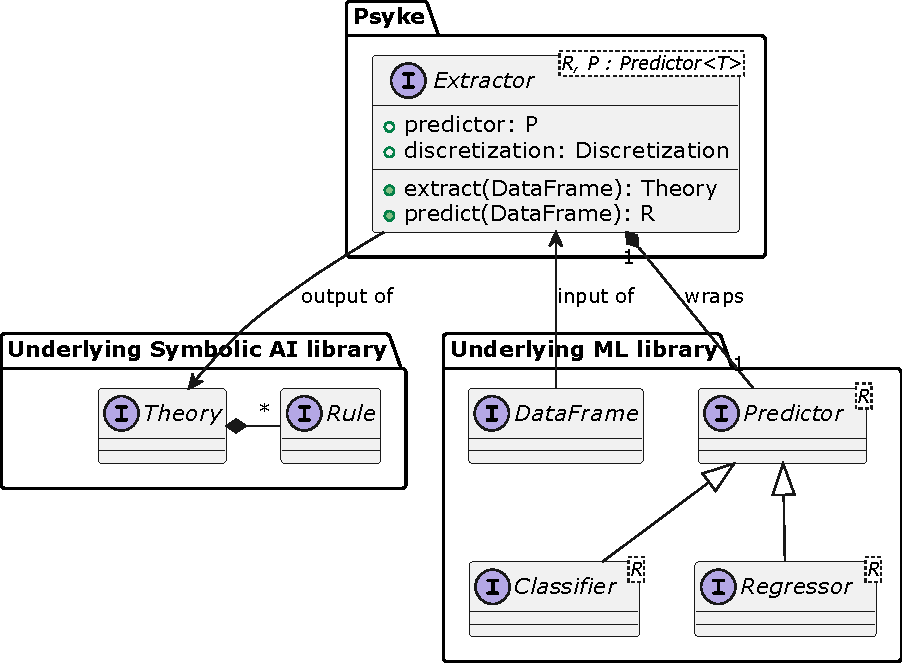
\includegraphics[width=.7\linewidth]{figures/extractor-api.pdf}
    \end{center}

    \framebreak

    General assumptions:
    %
    \begin{itemize}
        \item underlying ML library (e.g. \scikit{}\ccite{PedregosaVGMTGBPWDVPCBPD11}), providing:
        %
        \begin{description}
            \item[\kt{DataFrame}] a container of tabular data
            \item[\kt{Predictor<R>}] a computational entity which can be trained (a.k.a.\ fitted) against a \kt{DataFrame} and used to draw predictions of type \kt{R};
            \item[\kt{Classifier<R>}] a particular case of predictor where \kt{R} represents a type having a finite amount of admissible values;
            \item[\kt{Regressor<R>}] a particular case of predictor where \kt{R} represents a type having a potentially infinite (possibly continuous) amount of admissible values.
        \end{description}

        \framebreak

        \item underlying symbolic AI library (e.g. \twopkt{}\ccite{2pkt-swx16}), providing:
        %
        \begin{description}
            \item[\kt{Rule}] a semantic, intelligible representation of the function mapping \kt{Predictor}'s inputs into the corresponding outputs, for a particular portion of the input space;
            \item[\kt{Theory}] an ordered collection of rules.
        \end{description}
    \end{itemize}
\end{frame}

\begin{frame}[allowframebreaks]{About the Extracted Knowledge}

    \begin{block}{Knowledge extracted from \textbf{classifiers}}
        \begin{equation*}
            \begin{array}{rcl}
                \logicrule{\meta{task}(\var{X}_1, \ldots, \var{X}_n, \alert{\const{y}_1})}{p_{1,1}(\bar{\var{X}}),\ \ldots,\ p_{n,1}(\bar{\var{X}})}.
                \\
                \logicrule{\meta{task}(\var{X}_1, \ldots, \var{X}_n, \alert{\const{y}_2})}{p_{1,2}(\bar{\var{X}}),\ \ldots,\ p_{n,2}(\bar{\var{X}})}.
                \\
                & \vdots
                \\
                \logicrule{\meta{task}(\var{X}_1, \ldots, \var{X}_n, \alert{\const{y}_m})}{p_{1,m}(\bar{\var{X}}),\ \ldots,\ p_{n,m}(\bar{\var{X}})}.
            \end{array}
        \end{equation*}
    \end{block}

    \framebreak

    \begin{block}{Knowledge extracted from \textbf{regressors}}
        \begin{equation*}
            \begin{array}{rcl}
                \logicrule{\meta{task}(\var{X}_1, \ldots, \var{X}_n, \var{Y})}{p_{1,1}(\bar{\var{X}}),\ \ldots,\ p_{n,1}(\bar{\var{X}})},
                \\
                & & \alert{\var{Y}\ \const{is}\ f_1(\bar{\var{X}})}.
                \\
                \logicrule{\meta{task}(\var{X}_1, \ldots, \var{X}_n, \var{Y})}{p_{1,2}(\bar{\var{X}}),\ \ldots,\ p_{n,2}(\bar{\var{X}})},
                \\
                & & \alert{\var{Y}\ \const{is}\ f_2(\bar{\var{X}})}.
                \\
                & \vdots
                \\
                \logicrule{\meta{task}(\var{X}_1, \ldots, \var{X}_n, \var{Y})}{p_{1,m}(\bar{\var{X}}),\ \ldots,\ p_{n,m}(\bar{\var{X}})},
                \\
                & & \alert{\var{Y}\ \const{is}\ f_m(\bar{\var{X}})}.
            \end{array}
        \end{equation*}
    \end{block}

    \framebreak

    \ldots where:
    %
    \begin{itemize}
        \item $\mathit{task}$ is the $(n+1)$-ary relation representing the classification or regression task at hand,
        \medskip
        \item each $\var{X}_i$ is a logic variable named after the $i^\mathit{th}$ input attribute of the currently available data set,
        \medskip
        \item $\bar{\var{X}}$ is the $n$-nuple $\var{X}_1, \ldots, \var{X}_n$,
        \medskip
        \item each $p_{i,j}$ is either a $n$-ary predicate expressing some constraint about one, two or more variables, or the \pl{true} literal---which can be omitted,
        \medskip
        \item $\const{y}_i$ is the output of the $i^{th}$ prediction rule,
        \medskip
        \item $f_j$ is an $n$-ary function computing the output value for the regression task in the particular portion of the input space handled by the $j^\mathit{th}$ rule, and
        \medskip
        \item $\var{is/2}$ is the well-known Prolog predicate aimed at evaluating functions.
    \end{itemize}

    \framebreak

    \begin{block}{Underlying assumptions}
        \begin{enumerate}
            \item the input space is \alert{partitioned} into a finite set of regions

            \item each region is \alert{assigned} with a particular outcome, namely:
            %
            \begin{itemize}
                \item a \alert{class}, for \alert{classification} problems
                \item a \alert{constant}, or a simpler function, for \alert{regression} problems
            \end{itemize}

            \item \alert{one rule} generated describing \alert{for each region} and its corresponding outcome
        \end{enumerate}
    \end{block}
\end{frame}

\subsection{Usage Examples}

\begin{frame}[allowframebreaks]{Iris (classification)}\centering

    \includegraphics[width=.6\linewidth]{figures/CLA/iris-samples.pdf}

    \framebreak

    \pythonimport[basicstyle=\tiny\ttfamily]{listings/iris.py}

    \framebreak

    \input{figures/fig-comparison.tex}

    \framebreak

    \input{tables/tab-comparison.tex}

    \framebreak

    \prologimport[caption={Rules extracted by \real{} from MLP}]{listings/iris-real.pl}

    \framebreak 

    \prologimport[caption={Rules extracted by \real{} from 5-NN}]{listings/iris-trepan.pl}

\end{frame}

\begin{frame}[allowframebreaks]{Combined Cycle Power Plant (regression)}\centering
    \includegraphics[width=.6\linewidth]{figures/REG/ccpp-samples.pdf}

    \framebreak

    \pythonimport[basicstyle=\tiny\ttfamily]{listings/ccpp.py}

    \framebreak

    \input{figures/fig-comparison-reg.tex}

    \framebreak

    \input{tables/tab-comparison-reg.tex}

    \framebreak

    \prologimport[caption={Rules extracted for a regression problem}]{listings/ccpp-iter.pl}

\end{frame}

%===============================================================================
\section{Discussion}
%===============================================================================

\begin{frame}{Notable Remarks}
    \begin{itemize}
        \item commitment to a particular output shape / expressiveness
        %
        \begin{itemize}
            \item to preserve both human- and machine-interpretability
            \item other syntaxes may exist
        \end{itemize}
        \item discretization of the input space
        \item discretization of the output space
        \item features should have semantics per se
        \item further refinements may be applied to rules
        \item rules constitute global explanations
    \end{itemize}
\end{frame}

\begin{frame}{Current Limitations}
    \begin{itemize}
        \item tabular data as input $\rightarrow$ doesn't really work with images
        \item high dimensional datasets $\rightarrow$ very large, poorly readable rules
        \item highly variable input spaces $\rightarrow$ many rules $\rightarrow$ poor readability
    \end{itemize}
\end{frame}

\begin{frame}{Future research activities}
    \begin{itemize}
        \item target images or highly dimensional data in general
        \item target reinforcement learning (when based on NN)
        \item target unsupervised learning
        \item design and prototype your own extraction algorithm
    \end{itemize}
\end{frame}

%===============================================================================
\section*{}
%===============================================================================

%/////////
\frame{\titlepage}
%/////////

%===============================================================================
\section*{\refname}
%===============================================================================

%%%%
\setbeamertemplate{page number in head/foot}{}
%/////////
% \begin{frame}[c,noframenumbering]{\refname}
\begin{frame}[t,allowframebreaks,noframenumbering]{\refname}
%	\tiny
    \scriptsize
%	\footnotesize
    \bibliographystyle{apalike-AMS}
    \bibliography{ise-lab-ske}
\end{frame}
%/////////

%%%%%%%%%%%%%%%%%%%%%%%%%%%%%%%%%%%%%%%%%%%%%%%%%%%%%%%%%%%%%%%%%%%%%%%%%%%%%%%%
\end{document}
%%%%%%%%%%%%%%%%%%%%%%%%%%%%%%%%%%%%%%%%%%%%%%%%%%%%%%%%%%%%%%%%%%%%%%%%%%%%%%%%
